% Generated by scripts/2026-10-21/extract_floats.py from paper/main_ko.tex; edit the full manuscript, not this file.
\begin{figure}[htbp]
\centering
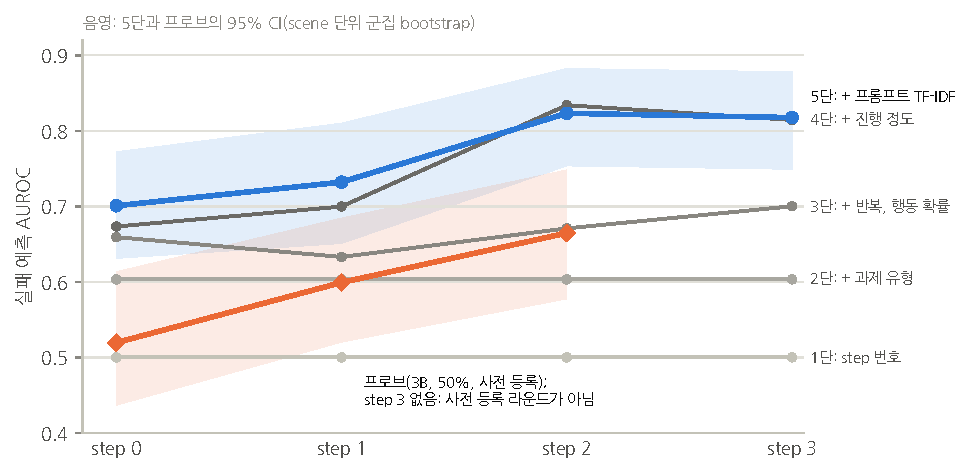
\includegraphics[width=\linewidth]{fig2_baseline_ladder_ko.pdf}
\caption{처음 250 episode에서 baseline 사다리(step 0--3)와 사전 등록 프로브(step 0--2)의 실패 예측 AUROC(step마다 $n = 250$, 실패 194). 5단과 프로브를 강조하고 scene 단위 군집 bootstrap(1,000회) 95\% CI를 음영으로 표시했다. 1--4단의 CI는 가독성을 위해 생략했다. 1단은 설계상 0.5이고 2단은 step에 따라 변하지 않는다. 두 음영이 겹치는지는 차이의 검정이 아니며, 짝지은 차이는 그림~\ref{fig:forest}에 있다.}\label{fig:ladder}
% 출처: results/baselines_main_3b.csv, results/probe_main_3b_primary.csv
\end{figure}
